% Simple article, but with some useful ApJ things included
% Created by AYQH, 18 June 2016
\documentclass[12pt, letterpaper, preprint]{aastex}
\bibliographystyle{apj}
\usepackage{float, bm, graphicx, subfigure, amsmath, morefloats, mathtools, amssymb}
\usepackage{color}
\usepackage{tabularx}

\setlength\parindent{0pt}

% useful macros
\newcommand{\ledd}{L_{\mathrm{Edd}}}
\newcommand{\medd}{\dot{M}_{\mathrm{Edd}}}
\newcommand{\Comment}[2]{ [{\color{red}\sc #1 :} {{\color{cyan} \it #2}}]}
\newcommand{\gcm}{g/$\mathrm{cm}^3$}
\newcommand{\angstrom}{\mbox{\AA}}
\newcommand{\vel}{\textbf{v}}
\newcommand{\bfield}{\textbf{B}}
\newcommand{\acc}{\textbf{a}}
\newcommand{\teff}{\mbox{$\rm T_{eff}$}}
\newcommand{\ncrit}{\mbox{$n_\mathrm{crit}$}}
\newcommand{\trelax}{\mbox{$t_\mathrm{relax}$}}
\newcommand{\nrelax}{\mbox{$n_\mathrm{relax}$}}
\newcommand{\tcross}{\mbox{$t_\mathrm{cross}$}}
\newcommand{\vrel}{\mbox{$v_\mathrm{rel}$}}
\newcommand{\rbondi}{\mbox{$r_\mathrm{Bondi}$}}




\begin{document}

\title{2015 ``Will Ask'' Qual Questions}

\section*{Radiative Processes}

\begin{enumerate}

  \item \textbf{Derive the total power and characteristic frequency 
      of synchrotron radiation from a relativistic particle of mass $m$, 
      charge $e$, and energy $E$ moving in a magnetic field $B$. 
      Use this to explain why synchrotron radiation is generally 
      negligible for protons.}

The total power is

\begin{equation}
  P = \frac{4}{3} \, \sigma_T \, c \, \gamma^2 \, \beta^2 \, u_B
  \label{eq:relativistic-larmor}
\end{equation}

where $\sigma_T$ is the Thomson cross section $\frac{8}{3} \pi r_0^2$,
$u_B$ is the magnetic energy density $\frac{B}{8 \pi}$.

The characteristic frequency of gyration is

\begin{equation}
\omega_g = \frac{eB}{\gamma mc}
\end{equation}

To derive this, begin with the equation of motion resulting from the Lorentz force:

\begin{equation}
  \frac{d}{dt} (\gamma m \vel) = \frac{e}{c} \, (\vel \times \mathbf{B})
  \label{eq:lorentz-force}
\end{equation}

For a particle with constant energy $E = \gamma m c^2$,
we can take $\gamma$ to be constant.
Therefore, Equation \ref{eq:lorentz-force} can be rewritten

\begin{equation}
  \frac{d \vel}{dt} = \frac{e}{\gamma m c} \, (\vel \times \mathbf{B})
  \label{eq:lorentz-force-rearranged}
\end{equation}

Because of the cross product in Equation \ref{eq:lorentz-force-rearranged}, the magnetic field only changes the component of the velocity that is perpendicular to it. Thus, Equation \ref{eq:lorentz-force-rearranged} can be rewritten

\begin{equation}
  \acc = \frac{d \vel_\bot}{dt} = \frac{e}{\gamma m c} \, (\vel_\bot \times \mathbf{B})
  \label{eq:lorentz-force-perp}
\end{equation}

Because $\vel_\parallel$ and $\vel_\mathrm{tot}$ are constant,
$\vel_\bot$ must be constant as well. Assuming an unchanging magnetic field, the acceleration in Equation \ref{eq:lorentz-force-perp} is constant. We thus have uniform circular motion in the ($\vel_\bot$, \bfield) plane. Together with the constant velocity normal to this plane, we have helical motion.

Because the motion is circular, the acceleration in Equation \ref{eq:lorentz-force-perp} can be taken to be a centripetal acceleration
with magnitude

\begin{equation}
a = v_\bot \omega_g = \frac{e v_\bot B}{\gamma m c}
\label{eq:acc}
\end{equation}

So, the corresponding characteristic frequency of rotation is

\begin{equation}
\omega_g = \frac{e B}{\gamma m c}
\end{equation}

To calculate the power, we use the \textbf{relativistic Larmor formula}
which gives the power radiated by a particle moving at relativistic speeds. It is derived via Lorentz transformations, taking the non-relativistic Larmor formula to hold true in the frame of the particle.
We use only one term of it, since the acceleration is perpendicular to the velocity.

\begin{equation}
  P = \frac{2}{3} \frac{\gamma^4 e^2 a^2}{c^3}
  \label{rel-larmor-formula}
\end{equation}

Now we plug in our expression for acceleration in Equation \ref{eq:acc} and average the formula over all angles (assuming an isotropic distribution of velocities). If $\alpha$ is the angle between the velocity of the particle and the magnetic field, 

\begin{equation}
\langle v_\bot^2 \rangle = \frac{v^2}{4 \pi} \int \sin^2 \alpha \, d\Omega
= \frac{2}{3} v^2
\end{equation}

With this averaging and some substitutions,

\begin{equation}
  P = \frac{4}{3} \, \sigma_T \, c \, \gamma^2 \, \beta_\bot^2 \, u_B
  \label{relativistic-larmor}
\end{equation}

The timescale on which power is lost due to sycnchrotron radiation
is about $\frac{E}{dE/dt}$. Since $E \sim \gamma m_0 c^2$ and
$ P = dE/dt$, we find that the timescale scales as $\gamma$. 
$\gamma$ itself scales as $E/E_0$ where $E_0$ is the rest mass energy
of the particle. This is roughly 0.511\,MeV for an electron and 938\,MeV
for a proton. So, for a given energy, the timescale is much longer
for a proton than it is for an electron.

Also, note that $\omega_g$ is not actually the frequency of radiation.
In practice, the frequency spectrum is complex and can extend up to many times $\omega_g$. Important effects include: 

\begin{itemize}

\item 
Broad spectrum due to relativistic beaming: the particle's radiation is beamed within $1/\gamma$ of a cone with half-angle equal to the pitch angle. This cone is the characteristic angular distribution of radiation emitted by a particle with perpendicular acceleration and velocity. Thus, instead of a sinusoidal light curve, you get a series of sharp pulses. Recall that the Fourier Transform of a short time pulse is a broad frequency spectrum with $\Delta \omega \sim 1/T$.

\item
The time between pulses is a factor of $\gamma^3$ narrower than what you'd get from $\omega_g$ due to the Doppler effect. 

\item
The single-particle spectrum extends to
something of order $\omega_c$ before falling away,
where $\omega_c \sim \gamma^3 \omega_g$. 

\item
The spectrum of a distribution of a population of relativistic electrons can be approximated by a power law over a limited range of frequencies. For a power law distribution of particle energies with index $p$ (that is, $N(E) dE = C E^{-p} dE$) over a sufficiently broad energy range, the spectral index of the radiation is $s = (p-1) / 2$. 

\end{itemize}

\newpage

  \item \textbf{Explain the connection between detailed balance, 
    the Einstein A and B relations,
    Kirchoff's law and the Milne relations, 
    and give an example of their use to connect the
    bremsstrahlung emission spectrum and the free-free absorption coefficient.}
    
\textbf{Detailed balance relations} govern the relationship between inverse processes on an atomic scale.
These processes could be transitions between atomic states
(the \textbf{Einstein A and B relations})
or photoionization and recombination (the \textbf{Milne relations}).
These atomic relationships are indifferent to whether the system is in thermal equilibrium: they don't care about the distribution of the intensity of radiation or the velocities of particles.
And yet, they are intimately connected to macroscopic-level relationships that \emph{do} depend on thermal conditions.
For example, the Einstein A and B relations
are implied by the macroscopic relationship between
emission and absorption (\textbf{Kirchoff's Law}).
Similarly, the \textbf{Bremsstrahlung emission spectrum} 
is intimately connected with absorption on an atomic scale characterized by the \textbf{free-free absorption coefficient}.

Here are the relations in more detail.

To understand the \textbf{Einstein A and B relations},
consider a system with two discrete energy levels 
$L_1$ and $L_2$ with statistical weights $g_1$ and $g_2$ respectively. To move between $L_1$ and $L_2$, the system
can do three things: emit a photon in the absence of a radiation field (spontaneous emission), absorb a photon (absorption),
or emit a photon in the presence of a radiation field (stimulated emission). The transition probability per unit time of these three processes are atomic properties, characterized
by the Einstein coefficients $A_{21}$, $B_{12}$, and $B_{21}$ respectively. The relations between these coefficients are: 

\begin{equation}
  g_1 B_{12} = g_2 B_{21}
  \label{einstein-B}
\end{equation}

\begin{equation}
  \frac{A_{21}}{B_{21}} = \frac{2 h \nu^3}{c^2}
  \label{einstein-A}
\end{equation}

To derive these relations, one invokes three consequences of thermodynamic equilibrium. 
The first is that the number of transitions into an atomic state is equal to the number of transitions out of that state:

\begin{equation}
  n_1 B_{12} \bar{J} = n_2 B_{21} \bar{J} + n_2 A_{21}
  \label{detailed-balance}
\end{equation}

where $\bar{J}$ is the intensity of the radiation field
weighted by the importance of different frequencies
in causing transitions (in practice, ``weighted" means
integrated over the line profile function):

\begin{equation}
  \bar{J} \equiv \int_0^\infty J_\nu \, \phi(\nu) \, d\nu
  \label{jbar}
\end{equation}

The second is that the relative number densities in the two levels are governed by the Boltzmann Equation:

\begin{equation}
  \frac{n_1}{n_2} = \frac{g_1}{g_2} \, e^{h \nu / k_B T}
  \label{boltzmann-eq}
\end{equation}

And the third is that $J_\nu = B_\nu$ and, further, since
$B_\nu$ varies slowly on $\Delta \nu$, that $\bar{J} = B_\nu$. 

Note that even though we invoke thermal equilibrium to derive these relations, the relations themselves have no dependence on temperature and thus hold regardless of whether the atoms are in thermal equilibrium. They are an extension of the law governing matter in thermodynamic equilibrium on a macroscopic scale, known as...

\textbf{Kirchoff's law for thermal equilibrium}
says that a blob of material at thermal equilibrium
(a blob whose emission depends solely on its temperature
and internal properties)
has a source function that obeys a blackbody spectrum.
In other words, the emitting and absorbing properties
of such a blob encourage radiation to approach
the Planck function $B_\nu(T)$.
More formally, this law relates
the material's absorption coefficient $\alpha_\nu$
to its emission coefficient $j_\nu$
and its temperature $T$:

\begin{equation}
  j_\nu = \alpha_\nu B_\nu (T)
  \label{kirchoff-law}
\end{equation}

This says that a good emitter is a good absorber, in
thermal equilibrium.

The \textbf{Milne Relations} govern the relationship between
photoionization and its inverse, radiative recombination.
In radiative recombination, an ion captures an electron
into a bound state $n$ and emits a photon. 
Just like we did for the Einstein relations
we use four consequences of thermal equilibrium to
derive a result that is independent of thermal equilibrium. 

The first consequence
is that the velocities of the electrons obey
a thermal distribution:

\begin{equation}
f(v) = 4 \pi \left( \frac{m}{2 \pi kT} \right)^{3/2} v^2 e^{-mv^2 / 2 kT}
\end{equation}

The second consequence is that the intensity of the radiation field is the Planck function $B_\nu (T)$.

The third consequence is that the relative number densities of ions $N_+$, electrons $N_e$, and neutron atoms $N_n$ are governed by the Saha equation:

\begin{equation}
\frac{N_+ N_e}{N_n} = \left( \frac{2 \pi m k T}{h^2} \right)^{3/2} \frac{g_e g_+}{g_n} e^{-\chi / kT} 
\end{equation}

Finally, the number of recombinations per time per volume due to thermal electrons is equal to the number of photoionizations per time per volume for a blackbody radiation field:

\begin{equation}
N_+ N_e \sigma_{fb} f(v) v dv = 
\frac{4 \pi}{h \nu} N_n \sigma_{bf} (1-e^{-h\nu/kT}) B_\nu d\nu
\end{equation}

where $\sigma_{fb} (v)$ is the cross-section for recombination
and $\sigma_{bf} (v)$ is the cross-section for photoionization.

Using these four properties together, we obtain the Milne relation:

\begin{equation}
\frac{\sigma_{bf}}{\sigma_{fb}} = \left(\frac{mcv}{h\nu} \right)^2 \frac{g_e g_+}{2 g_n}
\end{equation}


Now, let's turn to the application of these relations
to connecting \textbf{the Bremsstrahlung emission spectrum}
to \textbf{the free-free absorption coefficient}.
\textbf{Bremsstrahlung}, or \textbf{free-free emission},
is radiation due to the acceleration of a charge in the Coulomb field of another charge. For example, an electron under the influence of an ion's Coulomb field accelerates and radiates; the ion is much more massive than the electron and therefore its acceleration and radiation are negligible and for practical purposes its Coulomb field can be considered fixed.

You need quantum mechanics to fully understand this process, because the energies of the photons produced are comparable to that of the particle being accelerated. However, in some regimes you can justify a classical treatment to achieve the correct functional dependence, then make up for leaving out quantum mechanics by tacking on corrections called Gaunt factors. 

One such regime is the small-angle scattering regime, in which the electron's path is basically straight because the electron is moving so rapidly. In this regime, you can calculate the change in the electron's energy over the course of the time it spends closely interacting with the ion. In thermal conditions, you can integrate the resulting emission spectrum over a thermal distribution of particle speeds. Here is the resulting emission spectrum for \emph{thermal Bremsstrahlung}:

\begin{equation}
  \frac{dW}{dt dV dv} = \epsilon_\nu^{ff} = 4 \pi j_\nu^{ff} 
  = 6.8 \times 10^{-38} \, T^{-1/2} Z^2 n_e n_i \, e^{h \nu / kT}
  \, \bar{g}_{ff} (\nu,T)
  \label{eq:bremsstrahlung}
\end{equation}

Now, we do what we did before: relate a macroscopic process to an atomic process. In this case, the atomic process is thermal free-free absorption, the absorption of radiation by an electron moving in the field of an ion. Kirchoff's law tells us that

$$ j_\nu^{ff} = \alpha_\nu^{ff} B_\nu (T) $$

Using Equation \ref{eq:bremsstrahlung} we can solve for $\alpha_\nu^{ff}$, the free-free absorption coefficient:

\begin{equation}
\alpha_\nu^{ff} = 3.7 \times 10^8 \, T^{-1/2} Z^2 n_e n_i \nu^{-3} \, (1-e^{-h\nu/kT}) \, \bar{g}_{ff}
\end{equation}

In the Wien limit, $\alpha_\nu^{ff} \propto \nu^{-3}$.
In the RJ limit, $\alpha_\nu^{ff} \propto \nu^{-2}$.
So, low energy (low frequency) electrons are
preferentially absorbed. 

\newpage

\item \textbf{Draw the energy levels of the hydrogen atom and identify which transitions are allowed. Which ones are in the visible part of the spectrum? Which level has no allowed decays, and what is its main decay mode?}

The energy levels of the hydrogen atom are set by the following:

\begin{equation}
E = -13.6 \, \mathrm{eV} \left[ \frac{1}{n_1^2} - \frac{1}{n_2^2} \right] 
\end{equation}

\begin{center}
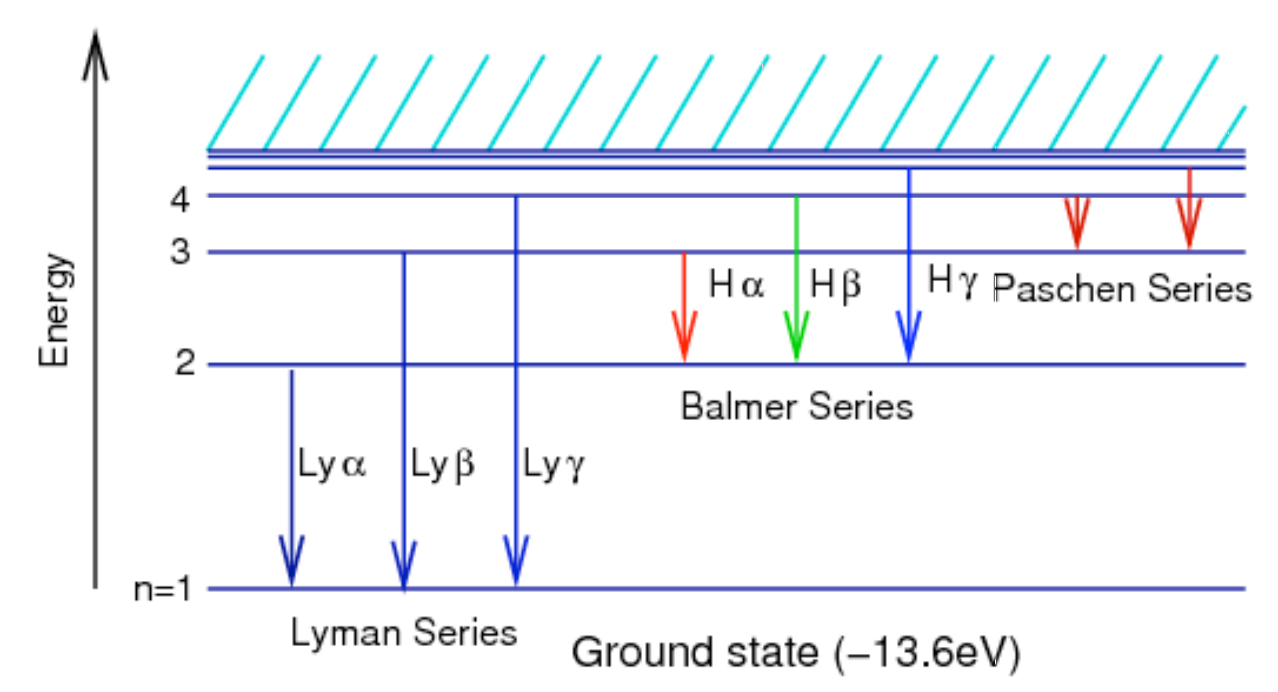
\includegraphics[scale=0.55]{hydrogen_atom_energy_levels.png}

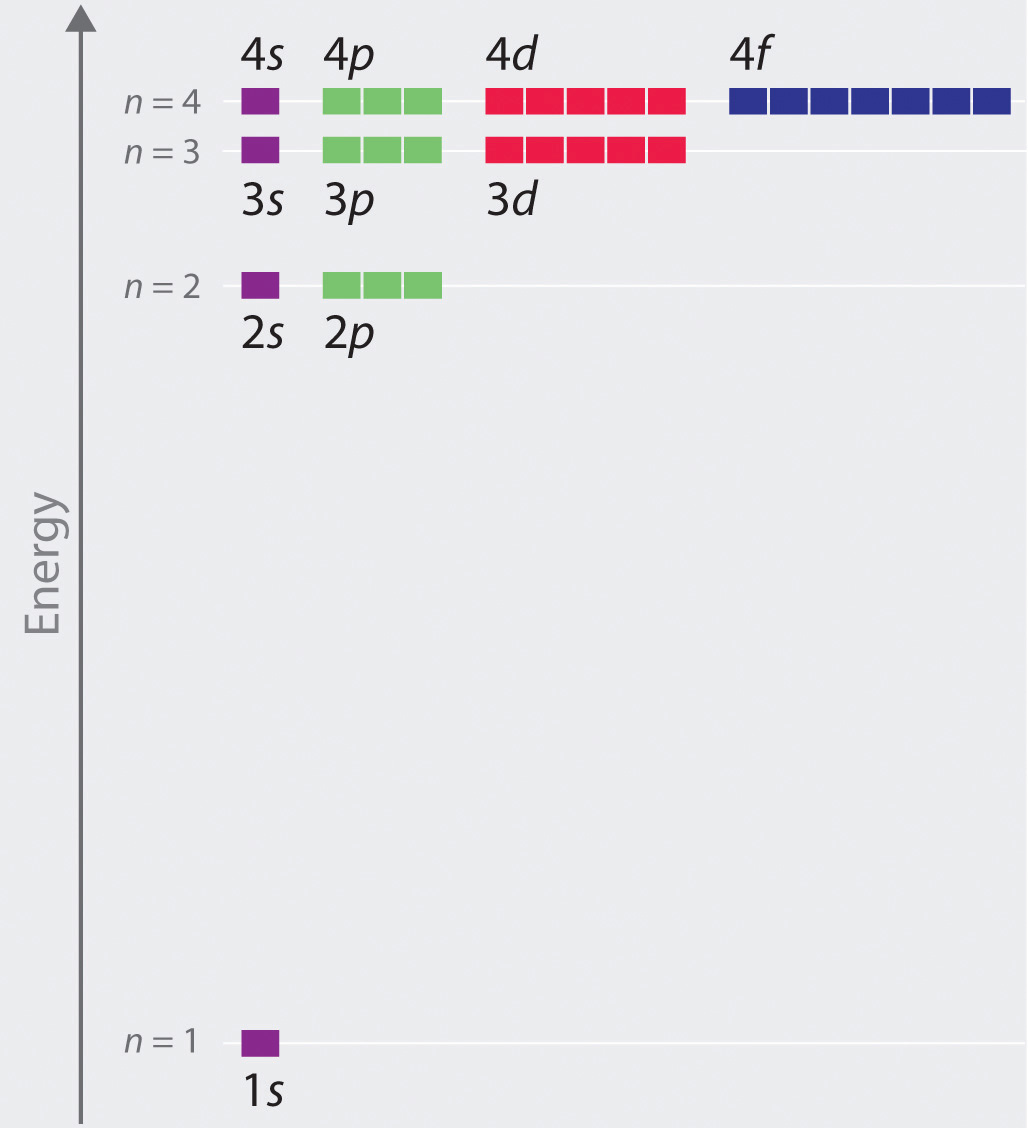
\includegraphics[scale=0.25]{hydrogen-atom-orbitals.jpg}
\end{center}

To determine which transitions are \emph{allowed},
we take some approximation scheme and identify which transitions would be strictly forbidden if that scheme were strictly true; thus, ``forbidden'' really just means ``highly improbable.''
Rules defined in this way are called \textbf{selection rules}.
In this case, we consider electric dipole transitions.
Thus, we set the transition probability to zero under the dipole approximation, which governs the perturbation from the external field: for $\mathbf{A}(\mathbf{r},t) = \mathbf{A} (t) \, e^{i \mathbf{k} \cdot \mathbf{r}}$, the approximation is that $e^{i \mathbf{k} \cdot \mathbf{r}} = 1$ which is equivalent to the limit that $v/c \ll 1$ for the electrons in the atom.
Bear in mind that the ``forbidden'' transitions defined this way could be nonzero for higher order multipole radiation or two-photon emission. 

The selection rules and the dipole approximation are part of a semi-classical theory of radiation: the atom is treated quantum mechanically but the impinging radiation field is treated classically. This is justified in the regime where the number of photons per photon state is large, so it describes induced processes but not spontaneous processes.

First, a quick refresher of how to treat the hydrogen atom quantum mechanically.
For a symmetric central potential, the eigenfunctions of an electron are

\begin{equation}
\psi_{n \ell m} (r, \theta, \phi) = r^{-1} R_{n \ell}(r) Y_{\ell m}(\theta, \phi)
\end{equation}

For a bound electron, $R_{n\ell}^2\,dr$ is the probability of being between $r$ and $r+dr$. $Y_{\ell m}(\theta, \phi)$ are the spherical harmonics,
eigenfunctions of the orbital angular momentum operator:

\begin{equation}
\mathbf{L}^2 Y_{\ell m} = \ell (\ell + 1) Y_{\ell m}
\end{equation}

\begin{equation}
L_z Y_{\ell m} = m Y_{\ell m}
\end{equation}

An \textbf{orbital} is essentially a spatial probability distribution governing the electron's location. It is fully characterized by three quantum numbers: $n, \ell, m$. Each orbital contains a maximum of two electrons, each distinguished by its spin $m_s$. 

$n = 1, 2, 3, ...$ is the \textbf{principal quantum number}, and describes the orbital SIZE (the energy shell/level/state).

$\ell = 0, 1, 2, 3, n-1$ is the \textbf{angular/orbital quantum number}, and describes the orbital SHAPE. Its values correspond to
$s, p, d, f, ...$ states. 

$m = -\ell, ..., +\ell$ is the \textbf{magnetic quantum number}, and describes the orbital ORIENTATION. 

Now, let's turn to transition probabilities. The transition probability under the dipole approximation contains the term: 

\begin{equation}
\mathbf{d}_{fi} \equiv e \int \phi_f^* \, \Sigma_j \,  \mathbf{r}_j \, \phi_i \, d^3 x
\label{eq:dipole-element}
\end{equation}

This dipole matrix element will involve the radial integral (shown below) as well as an integral over spherical harmonics.

\begin{equation}
\int r \, R_{nl} \, R_{n' l'} \, dr
\end{equation}

\begin{description}

\item[Laporte's Rule:]
There are no transitions between states of the same parity.
Looking at Equation \ref{eq:dipole-element}, we see that if
$f$ and $i$ have the same parity $(-1)^{\Sigma \ell_i}$,
the integral must vanish. 
That means that the configuration must change by at least one orbital.

\item[One-Electron Jump Rule:] The configuration must change by precisely one orbital.
Looking at Equation \ref{eq:dipole-element}, it can be written as a sum of matrix elements, each corresponding to a single product of wavefunctions: the sum will vanish unless all orbitals are the same except for one. 
Since transitions involve one electron at a time,
$\ell_i$ must change by $\pm 1$.

\item[For a single electron system:] From the integral over spherical harmonics involved in the dipole matrix element,
$\Delta l = \pm 1$ \& $\Delta m = 0, \pm 1$.

Since we're talking about the hydrogen atom, we're not worried about the many electron case. If we did worry about it, we'd be dealing with the total quantities $L, S, J$.
$\Delta S = 0$, $\Delta L = 0, \pm1$, $\Delta J = 0, \pm 1$. 

\end{description}

The Balmer lines (transitions to $n=2$)
are in the visible part of the spectrum. 

The 2s level has no allowed decays, because from 2s to 1s both the initial and final state have zero angular momentum. Each photon must carry angular momentum of at least one, so the 2s state cannot decay to the 1s state by emitting a single photon. So, for the 2s state to decay to the ground state, it has to emit two photons. The dominant contribution comes from two photons where their angular momenta cancel and are therefore in the $ J = 0 $ configuration. The decay rate is very small, smaller than the dipole transition from 2p to 1s by eight orders of magnitude. So, the 2s state is said to be metastable.
    
\end{enumerate} \newpage

\section*{Instrumentation}

\begin{enumerate}
\item \textbf{Describe quantitatively the point spread function 
of a diffraction-limited optical telescope. 
Explain how diffraction spikes arise, 
and what determines their position and intensities. 
Under what circumstances will the PSF be broadened by atmospheric
turbulence?}

Consider the path of a spherical wavefront (surface of constant phase) from a point source:
it expands, gets truncated by a finite aperture size,
diffracts around the edge of the pupil, then converges to a point. 
This diffraction sets a fundamental limit to the angular resolution that the telescope can achieve: the \textbf{diffraction limit.}

If a telescope is \textbf{diffraction limited},
then the optics are ``perfect'' and induce no wavefront aberrations.
For a diffraction-limited optical system, the 2D intensity distribution of the diffraction pattern at the image plane for a point source in the object plane is the
\textbf{point spread function (PSF)}.

For an optical system with a circular aperture, like most telescopes, the PSF is an \textbf{Airy diffraction pattern}, a Bessel function of the first order:

\begin{equation}
I = \left[ \frac{2 J_1 (r)}{r} \right]^2
\end{equation}

The Airy diffraction pattern is a series of nested rings centered on a bright spot called the \textbf{Airy disk}. Extra departures from this diffraction limited case will cause more light to be diffracted outside of the central peak, worsening the PSF.
In addition, real telescopes do not have purely circular apertures. The effect of a central obscuration is to decrease the amount of light in the central peak and increase the intensity in the diffraction rings.

The \textbf{Rayleigh criterion} says that two objects can be resolved when the central max of one PSF (one diffraction pattern) falls inside the first minimum of the other: 

\begin{equation}
\theta_\mathrm{min} = 1.22\,\frac{\lambda}{D}
\label{diffraction-limit}
\end{equation}

where D is the aperture diameter. 

\textbf{Diffraction spikes} arise from \textbf{spider vanes},
the support structures for the secondary mirror (a central obscuration), as you often have in a Cassegrain. These supports cast a shadow over the aperture and diffract the incoming light, and are manifested in the PSF as the spikes seen in images of bright stars.
Their position and intensities are determined by the number shape of the support bars: three vanes cause a six-spike pattern, four vanes cause a four-spike pattern,
and more area blocked corresponds to more intensity taken away from the main peak and shifted to outer parts of the pattern.
Wider vanes correspond to higher spike peak intensity and shorter spike length.
More quantitatively, the PSF is the Fourier Transform of the aperture function, intuitively because propagation of light through an optical system is reversible.
You can minimize this effect by using a support structure that casts a curved pattern on to the mirror. 

The spider diffraction effect is often illustrated by the effect of a narrow slit. The PSF caused by a slit apertureis $I(\theta) = \textrm{sinc}^2 (\beta) = \left( \frac{\sin \beta}{\beta} \right)^2 $. This sets the maxima and minima of the spikes. If the slits are fat, then you can approximate them as rectangular apertures, in which case this becomes the product of two sinc functions, one for the width and one for the length.

The PSF will be broadened by atmospheric turbulence under...most real-life circumstances; most observations are actually \textbf{seeing-limited} rather than diffraction-limited. 
Quantitatively, the onset of turbulence is $R_e = VL/v > 2000$ where
$V$ is the flow velocity, $L$ is the characteristic length, and $v$ is the viscosity, which is $1.5 \times 10^{-5}$ meters squared per second in air.

Basically, a wavefront is in practice not flat, becauase
light is refracted by the atmosphere and subjected to unevenness in temperature.
The boundary layer of the atmosphere is prone to wind turbulence, and there's turbulence due to air flow around the dome. There's also
a temperature gradient across height of the observatory. 

Turbulence is quantified by the \textbf{Fried parameter} $r_0$ which is the characteristic size of a turbulence cell, roughly 10 inches at a good site. Smaller $r_0$ corresponds to stronger turbulence. It gets smaller at shorter wavelengths and as the telescope looks towards the horizon due to the larger zenith angles. 

When there's turbulence, the wavefront gets out of phase and
the image size of a point source (PSF) is broadened: $\lambda/r_0 \gg \lambda / D$ assuming that $ D \gg r_0$. 

In practice, to achieve the diffraction limit, any departures from a perfect figure should be a fraction of the shortest $\lambda$ that will be observed. A truly diffraction-limited optical system would have 20-30\,nm residual wavefront error for UV/blue, but
for wavelengths shorter than 10\,$\mu$m, essentially no ground-based telescopes have achieved diffraction-limited images without adaptive optics. With Palomar you don't get anywhere close. At longer wavelengths, it's more feasible to correct for the atmosphere and push to the diffraction limit.
In the last 15 years or so, it has been realized that with careful control over thermal effects in domes, the best astronomical sites can deliver images with FWHM about 0.3 arcseconds even in the visible.
Solutions to the seeing problem: get above the atmosphere, or correct for it (Adaptive optics). 

\end{enumerate}

\section*{Stars}
\begin{enumerate}

  \item \textbf{Explain what the Hayashi track is, 
      and describe what types of objects live on it.
      Qualitatively explain how it arises and what 
      assumptions are required for its derivation.}
      
A \textbf{Hayashi track} is the steep (nearly vertical) loci in the HR ($\log \teff, \log L$) diagram of fully convective stars with a given mass and chemical composition. Tracks for increasing $M$ lie further to the left.

For certain stars, these tracks describe the path of a collapsing proto-stellar cloud, which you can think of as a contracting polytrope without nuclear energy sources. It may be shown that such a star is almost completely convective and hence, during its evolution, the luminosity decreases with decreasing radius while \teff is almost constant. So, the evolution takes place along an almost vertical track in the (log \teff, log $L_s$) diagram. The location of the track depends little on $M$.
This track is also significant for the later evolution of stars, clearly reflected by observed features (e.g. ascending branches of HR diagrams of GCs).

Each track represents a border between an allowed and forbidden region. Because the lines are so steep, you can think of this ``border'' as describing a minimum temperature:

\begin{equation}
\teff_\mathrm{min} = 4000\,K \mu^{13/51} \left( \frac{M}{M_\odot} \right)^{7/51} \left( \frac{L}{L_\odot} \right)^{1/102} 
\end{equation}

Note that the 1/102 reflects the very weak dependence on luminosity that causes the lines to be nearly vertical. Below this temperature, stars can't survive for very long because of the rapid pace of hydrostatic and convective adjustment. Above it, a star will fall on a free-fall timescale onto the Hayashi track. The stars in the allowed region have a small core with radiative transport. Left of the HL we have $\Delta < \Delta_\mathrm{ad}$ (so, some part of the model is radiative), on it we have $\Delta = \Delta_\mathrm{ad}$, and to the right we have $\Delta > \Delta_\mathrm{ad}$. 

The stars that live on it are fully convective; that is, they are fully convective from their center to the photosphere, while only the atmosphere remains radiative. They have adiabatic interiors. They are in hydrostatic equilibrium with a fully adjusted convection; that is, convective elements retain the properties required of them by mixing-length theory, because the changes in the star's large-scale quantities are slow enough to give these elements time to adjust. Fully convective stars have low \teff\ and lower mass, and thus the lines lie far to the right on the HR diagram.

The Hayashi track arises when you consider a crude model for fully convective stars, split up the star into an interior convective region and radiative atmosphere, and force a continuous pressure across the interface. In the interior, you assume that $\Delta_\mathrm{ad} = d \ln T / d \ln P$ and that the value of $\Delta_\mathrm{ad}$ is constant all the way from the interior up to the photosphere. For this to be true, you have to make two approximations: neglect the depression of $\Delta_\mathrm{ad}$ in ionization zones (regions near the surface where H and He are partially ionized) and ignore the superadiabatic convection that takes place in the region immediately below the photosphere. This simple stratification allows you to write a simple relationship between pressure and temperature in the whole interior: $P = CT^{1+n}$. Now, above the photosphere, in the atmosphere, you assume you have a radiative atmosphere described by a simple absorption law of the form $\kappa = \kappa_0 P^a T^b$. At the interface, you solve for the pressure in both directions, from the atmosphere integrating the hydrostatic equation, and set them equal to each other. This gives you a point on the HR diagram for every value of $R$, for given $M$ and $\mu$.

Correcting for these approximations tends to increase \teff. And the whole uncertainty in the mixing-length theory of ineffective convection propagates to an uncertainty in the precise value of \teff. 
     
\begin{equation}
\frac{L_s}{L_\odot} \approx 0.03 \left( \frac{M}{M_\odot} \right)^{-7} \left( \frac{\teff}{2400\,K} \right)^{40} 
\label{eq:hayashi-track}
\end{equation}

A notable feature of this relation is the very large exponent on \teff. Hence stars of this type all have nearly the same effective temperature, which according to Equation \ref{eq:hayashi-track} is around 2400\,K. 

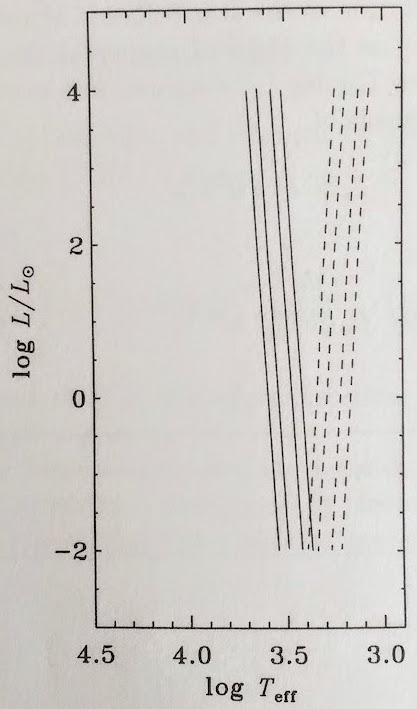
\includegraphics[scale=0.5]{hayashi-track.jpg}
     
  \item \textbf{Estimate the temperature as a function 
      of depth in the Sun’s convection zone.
      What is the temperature at the base of the convection zone?}
\end{enumerate} \newpage

\section*{Galaxies}

\begin{enumerate}

\item \textbf{Define two-body relaxation and estimate its time scale in (a) a globular cluster, (b) the Milky Way's disk. In which cases is two-body relaxation important?}

You can think of a galaxy in two ways:
a collisionless system in which particles move under the influence of a gravitational field that is generated by a smooth mass distribution,
or a collection of mass points in which the gravitational encounters between individual stars are dynamically important.
The characteristic \textbf{relaxation time} sets the boundary between these two regimes: for $t \leq \trelax$ the dynamics is governed by the former,
and for $t \geq \trelax$ the dynamics is governed by the latter. At this time, the star has essentially lost its memory of its initial conditions. Even though stellar collisions are extremely rare, the gravitational fields of passing stars exert a series of small tugs that slowly randomize the orbits of stars; gravitational encounters of this kind in a stellar system are analogous to collisions of molecules in a gas or Brownian motion of small particles in a fluid. All these processes drive the system towards energy equipartition and a thermally relaxed state.
In other words, we're answering the question of what happens to a star that's in some perpendicular orbit - what's the effect of the gravitational potential. The equation lets you calculate a timescale for relaxation, for energy redistribution and drive to equilibrium. 
Relaxation by gravitational encounters operates so slowly that it can generally be neglected in galaxies, except very close to their centers, but this process plays a central role in determining the evolution and present form of many star clusters. Two-body relaxation doesn't matter in galaxies because the stellar density is too low. 

\textbf{Two-body relaxation} is the process that becomes important at $t \geq \trelax$: the cumulative small kicks from many encounters with passing stars have changed the subject star's orbit significantly from the one it would have had if the gravitational field had been smooth. 
It is the diffusion of a star's velocity due to the cumulative effect of two-body encounters with the stars that it passes during its orbit, \emph{distinct} from the steady acceleration caused by the overall stellar mass distribution.

The \textbf{relaxation time} is a function of the number of stars in the system, as well as the \textbf{crossing time} $\tcross = R/v$, the time a typical star needs to cross the galaxy once:

\begin{equation}
\trelax \simeq \frac{0.1N}{\ln N} \tcross
\label{eq:trelax}
\end{equation}

In a globular cluster, $N \approx 10^5$ and the crossing time $\tcross \approx 1\,$Myr, which you can estimate from $r_h/\sigma_0$ where $r_h$ is the half-mass radius (3\,pc for a globular cluster) and $\sigma_0$ is the central velocity dispersion (6\,km/s for a globular cluster).
So, $\trelax$ is around a Gyr, significantly influencing the cluster structure over its lifetime of 10\,Gyr. 

In the Milky Way's disk, $N \approx 10^{11}$ and $\tcross \approx $. The thin disk has a radius of roughly $10^4\,$pc. Typical speed of a star on a circular orbit is 200\,km/s and it's useful to remember that 1\,km/s is almost exactly 1\,pc in 1\,Myr. The age of the galaxy is about 10\,Gyr so most disk stars have completed over forty revolutions and it's reasonable to assume that the Galaxy is now in an approximately steady state. Near the Sun, the random velocities of stars are typically about 50\,km/s. 
The disk is a few hundred crossing times old, so stellar encounters are unimportant, except very near the Galactic Center. 

You can derive Equation \ref{eq:trelax} using the following:

$$\trelax = \nrelax \tcross$$

where \nrelax is the number of crossings required for the star's velocity to change by of order itself. You can derive \nrelax by consider an individual star on its orbit around the galaxy. The question is: after one orbit, 
what is the order-of-magnitude difference between its actual velocity
and the velocity it would have had if the mass of the other stars were smoothly distributed? 

The velocity is expected to change, or be deflected, due to the interaction between the star and another star. Assume that the $\delta \mathbf{v}/v \ll 1$ so that the trajectory is straight, and that the star it is interacting with does not move. 

Here is the picture:

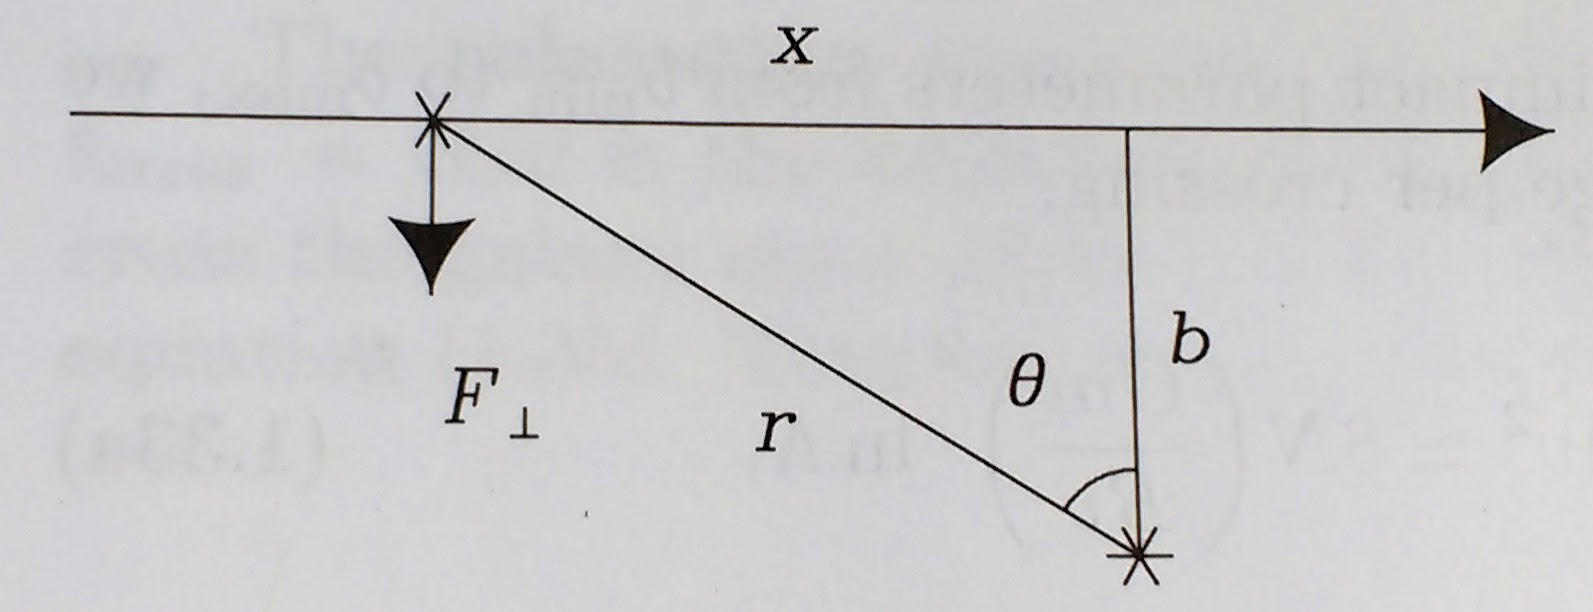
\includegraphics[scale=0.2]{2body-encounter.jpg}

$b_0 = \frac{2GM}{\vrel^2}$ is the \textbf{hard scattering} parameter. And the scattering cross section is $\sigma_0 = \pi b_0^2$. Note that the faster they're going, the less time they have to interact.
Integrate the perpendicular force $F_\perp$ to get
$\delta v$, the velocity deflection due to this single encounter with impact parameter $b$. 

\begin{equation}
\delta v = \frac{2GM}{bv}
\end{equation}

Think of this as the (acceleration at closest approach) times (duration of acceleration): in other words, we're assuming that all of the action happens in one impulse.
Then you calculate the number of encounters per impact parameter, and integrate over all of the impact parameters, from $b_\mathrm{min}$ to $b_\mathrm{max}$, letting
$b_\mathrm{min} \approx b_{90}$ and $b_\mathrm{max} \approx R$. From this, you get the mean square velocity change per crossing, and can find \nrelax:

\begin{equation}
\nrelax \simeq \frac{N}{8 \ln \Lambda}
\end{equation}

where $\Lambda = \frac{b_\mathrm{max}}{b_\mathrm{min}}
\simeq \frac{R}{b_{90}} \simeq \frac{R v^2}{GM} \simeq N$,
because $ v^2 \approx \frac{GNm}{R} $. 

From Chuck's notes: 
galaxies are quite easy to treat physically:
like a collisionless gas because stars don't go anywhere
near each other unless they're born that way.

\newpage

\item \textbf{Draw qualitatively the spectral energy distribution of the Milky Way, and describe how its morphology might appear to an external observer as a function of wavelength.}

Here's an SED of a massive, metal-rich star-forming galaxy (like ours). It's half optical (stellar black body) and half IR (dust black body). The shape is a mix of (broad) blackbodies and narrow features (lines). 
You get other shapes at very long wavelengths (synchrotron, free free). Millimeter and radio emission are footnotes, useful as a tracer of conditions.


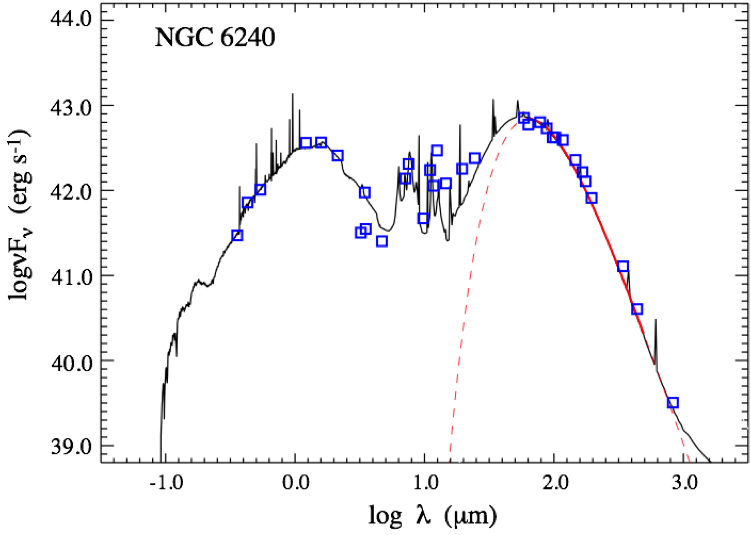
\includegraphics[scale=1.0]{sed.png}

And before we proceed, here's a quick cartoon for guidance:

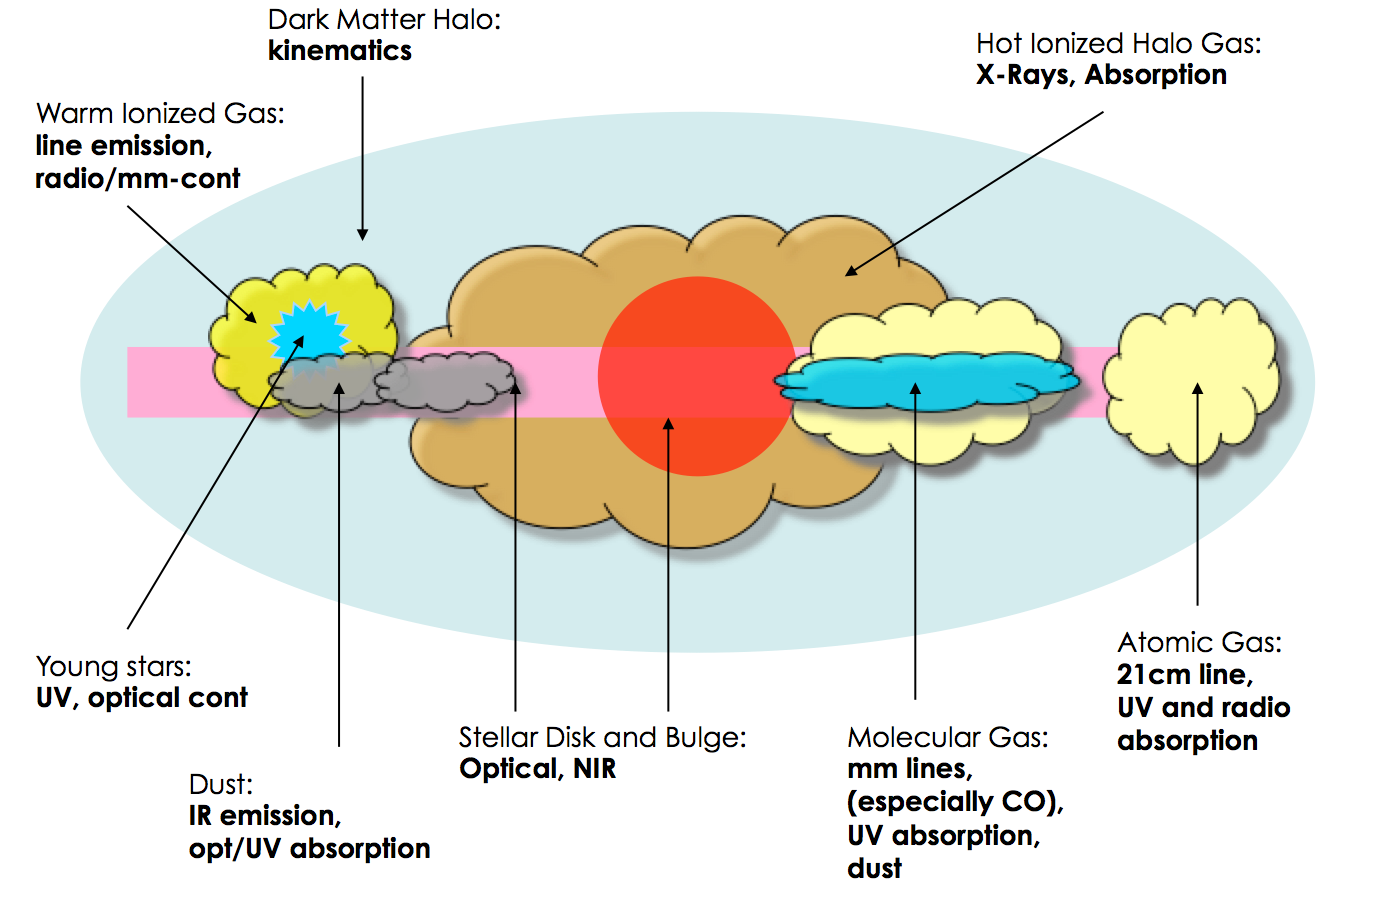
\includegraphics[scale=0.3]{galaxy-anatomy.png}

Let's take M51 as a counterpart.
\textbf{The spiral arms seen in dust, non-thermal radio continuum emission, and CO} mark the high-density gas arms caused by orbit crowding.
\textbf{The spiral arms in HI, young stars, and HII regions} lie outside the gas arms.
This is explained by density-wave theory: the displacement of the bright-star arms from the gas arms marks the time lag required for star formation. If the spiral is trailing, this displacement implies that the wave must be moving more slowly than the disk material.

\begin{description}
\item[Visible (blue):] The SED of a spiral galaxy is dominated by the light from luminous, young (blue) stars and HII regions. Baade (1963): the HII regions are ``strung out like pearls along the arms.'' Blue light traces star formation. Visible light traces the distribution of stars. Optical light dominated by markers of recent star formation: luminous blue stars and reddish HII regions.
\item[Near-IR, $3.6\,\mu$m:] absorption by dust much less severe, mostly due to giant stars continuously produced from the old MS dwarfs that dominate the mass. Contribution of young stars to the near-IR flux is small, except in localized regions of rapid SF. Thus, near-IR light traces mass. Spiral arms are smoother and broader because the irregular spatial distribution of star formation sites has been phase-mixed away in the old stars. The presence of spiral structure in the old stars that dominate the mass population is common and tells us that the entire stellar disk participates in the spiral pattern...there's a spiral pattern in both the surface density of the disk and in the star formation rate as seen in visible light. Usually, the arm traced by the young stars is displaced slightly inside the old-star arm. 
\item[Relativistic electrons, 6\,cm:] mainly synchrotron radiation, relativistic electrons. ISM in galaxies contains relativistic electrons and magnetic fields, so synchrotron radiation (mostly non-thermal radio emission). Compression of gas in spiral arms enhances $n_e$ and $B$ because the magnetic field is frozen into the interstellar gas. You see well-defined radio spiral arms lying inside the bright-star arms, magnetic field oriented along the arms. Although in a nearby grand-design spiral you might see radio arms that are broader and centered on the bright star arms, possibly because they are strongest where SNe remnants enhance $n_e$. Large-scale B fields are strongest in the interarm region. Relation of radio arms to other arm tracers remains a bit unclear. 
\item[Molecular gas like CO, 2.6\,mm:] CO luminosity probably traces total mass in molecular gas ($H_2$).
Narrow spiral arms coincide closely with the dust lanes, CO arms traces high-density gas. Enhanced CO emission comes from higher gas density that enhances the rate of collisional excitation and promotes the formation of new molecules.
\item[Neutral atomic gas, 21\,cm:] HI arms coincide with the bright-star arms, suggesting that enhanced density of HI comes not from gas compression, but from dissociation of molecular hydrogen by UV radiation from young stars formed in the arm. Thus in some cases the HI arms may be a product, rather than a precursor, of rapid SF. 21\,cm emission traces the distribution of neutral atomic hydrogen, found at much larger radii than the stars.
\item[HII regions, H$\alpha$ emission line of the Balmer series:] regions of ionized gas surrounding hot stars,
trace the bright-star spiral arms. 
\end{description} \newpage

\item \textbf{Describe at least three methods to probe the gravitational potential of galaxies, their assumptions, and their realm of applicability.}

To ``probe the gravitational potential of galaxies''
is to map out the distribution of mass,
including contributions from stars as well as
contributions from dark matter. 

Ideally, we would use dynamical modeling.
We would make models and compare them with observations of dynamical tracers like the velocity fields of gas and stars, and observations of gravitational lensing.
That said, dynamical tracers can only measure total mass;
they can't separate stellar and DM contributions.
In any case, at present, we are not in a position to do this. 

\begin{enumerate}

\item Radial velocity curves of spiral galaxies. 
Here you're assuming Keplerian motion of the stars in the disk and that you can easily obtain disk velocities from the radial velocity by knowing how the galaxy's plane is projected on the sky. Majority of constraints on the Galactic potential from Disk stars have been derived through the Jeans Equation (because one has a clear prior on the orbital structure: most orbits should be nearly-circular, deviations can be treated as vertical or in-plane oscillations). But this doesn't give you a distribution function for the stars and doesn't provide constraints on the potential marginalized over the possible distribution functions.
      
\item Velocity dispersions of ellipticals. Here you can use the width of spectral lines to find the velocity distribution of stars. Limited to ellipticals (and maybe bulges of spirals?). Vertical density distribution of tracer particles and their vertical velocity distribution...
      
\item Gravitational lensing. Use the angle that light is gravitationally bent (corresponding to the Einstein radius) to measure the mass of a galaxy or galaxy cluster. Usually it's harder to get detailed information about the potential in space, since you'll normally just have one or a few lensed objects behind your foreground object. You also need to pick a foreground objects with lensable objects behind it.

\end{enumerate}

\end{enumerate}

\newpage

\section*{High Energy}

\begin{enumerate}

\item \textbf{Derive, approximately or exactly up to dimensionless factors, the Bondi accretion rate onto a mass $M$ at rest in a homogeneous medium of density $\rho$ and speed of sound $c_s$. Explain the significance of the Bondi radius.}

\textbf{Bondi accretion} refers to steady, spherically symmetric accretion. For example, we can consider a star mass $M$ at rest with respect to the surrounding interstellar medium, accreting spherically symmetrically from the gas cloud around it.
To derive the accretion rate $\dot{M}$, we connect two environments:
the ambient conditions far away from the star,
and the conditions near the surface of the star.
More specifically, we assume that ambient conditions at infinity are characterized by $\rho$ and $c_s$, and that near the star 
the flow is supersonic: $v^2 > c^2$.
A steady accretion flow greater than or equal to this value muss possess a sonic point: that is, the inflow velocity must become supersonic near the stellar surface.
This \textbf{Bondi accretion rate} is:

\begin{equation}
\dot{M} = \pi \rbondi^2 c_s(\infty) \rho(\infty)
= 1.4 \times 10^{11} \left( \frac{M}{M_\odot} \right)^2 \left( \frac{\rho(\infty)}{10^{-24}} \right) \left( \frac{c_s(\infty)}{10\, \mathrm{km/s}} \right)^{-3} \mathrm{g/s}
\end{equation}

The significance of this \textbf{Bondi radius} is that it gives the range of influence of the star on the gas cloud. For $r \gg \rbondi$, the gravitational pull of the star has little effect on the gas: $c_s(r) \sim c_s(\infty)$. At this radius, a gas element of mass $m$ has roughly equal amounts of internal (thermal) energy and gravitational binding energy. The value is:

\begin{equation}
\rbondi = \frac{2GM}{c_s(\infty)^2} 
= 3 \times 10^{14} \left( \frac{M}{M_\odot} \right) \left( \frac{10^4\, \mathrm{K}}{T(\infty)} \right) \mathrm{cm}
\end{equation}

To do the derivation, begin with the Bernoulli Equation:

\begin{equation}
\frac{1}{2} u^2 + \int \frac{dP}{\rho} - \frac{GM}{r} = e = \mathrm{constant}
\end{equation}

Far away from the star, you can neglect the velocity $u$ because it goes as $\frac{1}{r^4}$. Out there, the conserved quantity is just the second two terms. You can write the first in terms of the sound speed:

$$ \int \frac{dP}{\rho} = \frac{1}{\gamma-1} c_s^2 $$

since $c_s^2 = \frac{\gamma P}{\rho}$. 

Thus, we have the conservation statement

$$ \frac{1}{\gamma-1} c_s^2 - \frac{GM}{r} = \frac{1}{\gamma-1} c_{s,\infty}^2 $$

The Bondi radius is where the sound speed has changed by order unity from its original value. And, it marks the transition from subsonic (far from the BH) to supersonic (close to the BH). 

At supersonic speeds, 

\begin{equation}
r_\mathrm{Bondi} = \frac{GM}{c^2_\infty}
\end{equation}

At this transition point, the mass accretion rate is governed by conservation of mass:

$$ \dot{M} = 4 \pi r^2 \rho u = 4 \pi \rho u \left(\frac{GM}{c^2_\infty}\right)^2 $$

With some fudge factor $\lambda$,

\begin{equation}t
\dot{M} = \lambda 4 \pi \left(\frac{GM}{c^2_\infty}\right)^2 \rho_\infty c_\infty
\end{equation}

\newpage

\item \textbf{Discuss the difference between high-mass X-ray binaries and low mass X-ray binaries (both containing neutron stars). What are the typical spin period and magnetic fields of the neutron stars in the two types of system, and how are these measured or estimated? How are the spin period and magnetic fields changing with time?}

In many X-ray binary systems, the spin period is observed to be decreasing steadily on a timescale of around 10,000 years. Presumably, this is caused by torques induced by the accretion process. Observed spin periods are usually between 1 second and 1000 seconds. 

Observe LMXB (accretion from Roche lobe overflow, orbital period hours) with coherent X-ray pulsing. The X-ray pulsing continues even when the X-ray intensity drops by large factors. Surface magnetic field of around $10^9$\,G, far lower than the fields inferred in pulsing sources in HMXB (accretion from the stellar wind of a massive (O or B) star, orbital period $\sim$months, $B \sim 10^{12}$\,G). May suggest that the fields decay, perhaps as a result of accretion. You can also measure weak magnetic fields from quasi-periodic oscillations detected in the power spectra of LMXBs. Spin period on the order of milliseconds. These are the progenitors of the majority of millisecond pulsars. 

HMXB systems emit x-ray pulsations, LMXB systems emit x-ray bursts.

\newpage

\item \textbf{Derive the equation for the effective temperature of an accretion disk around a black hole of mass $M$ with accretion rate $M_\odot$ as a function of radius $r$. Specify the assumptions required to get an answer, and comment on what could go wrong with them. Define the Eddington luminosity and explain its relevance to the peak frequency of the emitted radiation.}

Consider a fully ionized gas and assume it's unmagnetized. There's some flux coming in and on average, photons come out perpendicular. The Thompson cross section is

\begin{equation}
\sigma_T = \frac{8 \pi}{3} \left( \frac{e^2}{m_e c^2} \right)^2
\end{equation}

So the radiation force is

\begin{equation}
\mathrm{Force} = \sigma_T \frac{F}{c}
\end{equation}

Now, assume that for each electron, radiation force balances gravity ($m_e g$) and solve for the luminosity limit for keeping electrons bound:

$$ L_e < \frac{4 \pi G M m_e c}{\sigma_T} = 7 \times 10^{34} \left( \frac{M}{M_\odot} \right) \, \mathrm{erg/s}$$

There are lots of stars, white dwarfs, and neutron stars that have much higher luminosity than this. The mistake is that we assumed that only the gravitational force was acting, but there's also a (stronger) electric force:

$$ \frac{e Q}{r} > \frac{G M m_e} {r^2} $$

When this is the case, you can estimate the \emph{fraction} of electrons that are lost by the number of electrons lost over the total number of electrons: $\frac{Q/e}{M/m_p}$. You can write this in terms of the ratio of proton mass to electron mass and the fine structure constant. When you do, you find that the number is \emph{tiny}: the moral is that there aren't that many electrons to be lost. 

Instead of individual electrons, let's consider ions: you have to remove an entire ion with its electrons in order to unbind. The balance between gravitational force and radiation force becomes

$$ M_{\mathrm{ion}} g = F_{\mathrm{rad, ion}} $$

Since the electron mass is negligible compared to the proton mass, $M_{\mathrm{ion}} \sim A m_u$. $F_{\mathrm{rad, ion}}$ is just the sum of the radiation force on each electron, so $F_{\mathrm{rad, ion}} = Z F_{\mathrm{rad, e}}$. The maximum luminosity the star can have without losing ions to radiation is therefore: 

$$ A m_u \frac{GM}{r^2} > \frac{L}{4 \pi r^2 c} Z \sigma_T $$

This gives us our definition of the \textbf{Eddington luminosity}:

\begin{equation}
\ledd \equiv \frac{4 \pi G M c}{Z \sigma_T / A m_u} = \frac{4 \pi G M c}{\sigma_T (1 + X) / (2 m_u)}
\end{equation}

where $X$ is the hydrogen mass fraction. 

To estimate a numerical value for this, put it in terms of the $L_e$ that we solved for earlier, and the $m_p/m_e$ ratio. This gives:

$$ \ledd = 1.3 \times 10^{38} \frac{2}{1+X} \left( \frac{M}{M_\odot} \right) \mathrm{erg/s} $$

This could be violated under the following circumstances:

\begin{enumerate}
\item Different opacity: dust or photoionization (this is why red giants have enormous dusty winds) or strong magnetic fields (quantum electrodynamic effects).
\item Electrons are actually not bound; instead, they're flowing out due to a wind (radiation convection).
\end{enumerate}

When you accrete, you basically drop stuff onto a hard surface. The energy released is the change in potential energy $ \frac{G M \dot{M} }{R} $. In order to accrete, you must be radiating below $\ledd$; otherwise, the effective gravity would be in the other direction. So, $\ledd$ sets the maximum luminosity above which the object can no longer accrete. This therefore corresponds to a maximum mass accretion rate:

\begin{equation}
\medd \equiv \frac{4 \pi c R}{\sigma_T (1 + X) / 2 m_u}
\end{equation}

Numerically,

$$ \medd = 1.5 \times 10^{-8} \, \frac{M_\odot}{\mathrm{yr}} \left( \frac{R}{10\,\mathrm{km}} \right) \left( \frac{2}{1+X} \right) $$

\textcolor{red}{In short, radiation pressure on electrons balances with gravity on nuclei. $\mathrm{Force}=\mathrm{Flux} \times \bar{Z}\sigma_{T}/c=GM \bar{A}m_u/r^2$. For disk accretion, radiation is not necessarily to be isotropic. }

\end{enumerate}

\newpage

\section*{ISM}

\begin{enumerate}

\item \textbf{Discuss the principal heating mechanisms and cooling transitions which determine the temperature of the principal phases of the interstellar medium: cold molecular, warm neutral, warm ionized, and hot ionized.}

Each phase of the ISM has some equilibrium temperature: the \textbf{Cold Molecular Medium} around 10-50\,K, the \textbf{Warm Neutral Medium} around 5000\,K, the \textbf{Warm Ionized Medium} around $10^4$\,K, and the \textbf{Hot Ionized Medium} above around $10^{5.5}$\,K. When the temperature of the gas departs from these values, heating or cooling processes dominate until the temperature is restored to equilibrium.

A bit on each phase:
\begin{itemize}
\item The CMM consists of gravitationally bound clouds of H2, the sites of star formation. H2 molecules survive because the densities are high enough for self-shielding, although notes that the densities would still qualify as ultrahigh vacuum in a terrestrial lab. 
\item The WNM is predominantly HI gas that fills a significant fraction (maybe 40\%) of the disk volume.
\item The WIM consists of H II gas either in a dense cloud (``H II region'') or floating diffusely between clouds. The hydrogen gas was photoionized by UV photons from hot stars, primarily recently formed massive O stars. The dominant element, H, is nearly fully ionized. 
\item The HIM consists of coronal gas, shock-heated and collisionally ionized by blastwaves from supernovae. Most is low density and fills about half of the volume of the disk as well as much of the volume above and below it.
\end{itemize}

For all phases except the HIM, the dominant heating mechanism is \textbf{photoionization}. The idea is that electrons are freed from either dust grains or atoms, and their kinetic energy adds thermal energy to the gas. At lower temperatures (so, in the CMM and WNM) the photoelectrons come primarily from the surface of dust grains. These surface electrons are very loosely bound in the first place, so this process requires much less energetic photons ($h\nu > 8$\,eV) than the photoionization of atoms. At higher temperatures, in the WIM, photoelectrons come from H \& He atoms (this is what \emph{defines} an HII region) which requires energies above the ionization threshold 13.6\,eV. 

\begin{equation}
X^{+r} + h\nu \rightarrow X^{+r+1} + e^- + KE
\label{photoionization}
\end{equation}

Another important heating mechanism is \textbf{shocks} from supernovae and stellar winds; this often dominates or is at least comparable in the WNM, and \emph{is} dominant in the HIM. A bit on supernova shocks: the shock front comes from the fact that the velocity of the outermost ejecta is greater than the sound speed in the circumstellar medium. The ejecta within the shock front expands adiabatically and cools, but is then heated back up by the reverse shock triggered when the pressure of the shocked medium becomes larger than the thermal pressure of the outermost ejecta (around when the expanding material has swept up a mass of circumstellar/interstellar matter comparable to the ejecta mass).

In the WNM, other subdominant contributions come from \textbf{cosmic rays} and \textbf{hard x-rays} (although these are important if you're near an AGN). In the HIM, other subdominant contributions come from interactions with other regions, whether via \textbf{mergers}, \textbf{outflows}, or inflows (\textbf{accretion shocks}). 

For all phases, a dominant cooling transition is \textbf{collisionally excited metal lines}: lines from atoms that are collisionally excited and then radiatively decay. 
You can't collisionally excited H and He because the gap between states is too high, but metals (like oxygen) have ions (e.g. [O I], [O II], [O III]) with energy levels that can be collisionally excited by electrons with KE of just a few eV.
Some of these are fine structure transitions and some are transitions from electronic excited states. 
In the WNM, the dominant lines are [OI] at 63\,$\mu$m and [C II] at 158\,$\mu$m. In H II regions, the principal collisionally excited cooling lines are [N II], [O II], [O III], [Ne II], [S II], and [S III], stretching from the mid-IR through UV. The [S II], [N II], and [O II] lines are particularly prominent in the optical spectrum of an H II region.
Of course, there's no net effect if the collisional excitation is immediately followed by deexcitation.

Other cooling transitions in the WNM are \textbf{molecular CO}. 

Other important cooling mechanisms in the WNM are \textbf{thermal emission from dust}.

Other important cooling mechanisms in the WIM are \textbf{radiative recombination} (particularly of $\mathrm{H}^+$) and \textbf{free-free emission from free electrons}. The major hydrogen recombination lines $H \alpha$, $H \beta$, and $H \gamma$ dominate the optical spectrum of an H II region. 

In general, ionized plasma produce copious amounts of x-rays, which carry away significant quantities of energy. At very high temperatures ($T > 10^7$\,K) in the HIM, the dominant cooling mechanism is \textbf{x ray emission} from Bremsstrahlung. 

\newpage

\item \textbf{Explain how the temperature, density, ionizing spectrum and element abundances of an H II region can be estimated using measurements of different line transitions.}

The principle here is that populations of excited states of atoms and ions depend on the local density, temperature, and element abundances. So, these quantities can be estimated via measurements of the level populations of atoms and ions. Line transitions give you a way to probe these levels, assuming that the abundances and energies of the radiative transitions are practically suitable for observations. 

A key concept here is the \textbf{critical density:} the density at which collisional de-excitation and radiative de-excitation are equal. The density regime of the ionized region ($n_e \gg \ncrit$, $n_e \ll \ncrit$) determines what quantities can be inferred from the line ratios.

\textbf{Estimating Temperature}

In the regime where $n_e \ll \ncrit$, most atoms are in their ground state rather than being collisionally excited. If an atom has two excited levels at very different energies, you get two frequencies of observable line emission, with a relative strength sensitive to temperature.
In fact, in this density limit, \emph{temperature} is the only property of the gas that determines this emissivity ratio (obviously, it's also sensitive to atomic physics.) 

For species to be useful, its two excited levels must both be accessible at the temperatures of interest (so that there's significant emission),
and their energy difference must be comparable to $kT$ so that the populations are sensitive to the ambient temperature.
They must be readily abundant and not too easily photoionized;
the dominant process must be collisional excitation.
Useful species include [O III], [N II], and [S III]. 
A particular example is the line ratio [N II 5756] / [N II 6585]. 

You can also use the strengths of the discontinuities in the recombination continuum relative to the strengths of recombination lines.
The most commonly used such discontinuity is the \textbf{Balmer Jump}
at $\lambda = 3645.1$\,\AA. This is produced by recombining electrons with zero kinetic energy, and is therefore proportional to the electron energy distribution, so $T^{-3/2}$. To measure the jump, you pick two points: one blueward of this value, one redward of this value, both between H recombination lines. The ratio of this value to the strength of a recombination line like H11 will depend on temperature by something like $T^{-0.7}$, which is strong enough to be useful. 

Finally, you can observe lines emitted following excitation via \textbf{dielectronic recombination}. The ratio of lines due to dielectronic recombination to lines due to collisional excitation is temperature-dependent, because the rate coefficients for the two processes have different temperature dependencies. 

\textbf{Estimating Density}

In general, line ratios will have one value in the low density limit (where every collisional excitation is followed by spontaneous radiative decay) and another value in the high density limit (where levels are thermalized and populations are proportional to their degeneracies; relative populations are insensitive to temperature). In between, the ratio will be sensitive to the density.

In this regime, you can estimate density using ions with two or more energetically accessible energy levels that are at nearly the same energy, so that the relative rates for populating these levels via collisions are nearly independent of temperature. A common example is [O II], e.g. the line ratio [O II 3730] / [O II 3727]. 

You can also estimate densities via the \textbf{Balmer decrement}, a sequence of line ratios that are relatively insensitive to electron temperature but, at high densities, are affected by the density because of collisional effects, e.g.:

$\frac{I (H \alpha)}{I (H \beta)}$,
$\frac{I (H \gamma)}{I (H \beta)}$,
$\frac{I (H \delta)}{I (H \beta)}$ \newline

\textbf{Estimating Element Abundances}

To get the abundance of He relative to H, you compare the strengths of radiative recombination lines of H and He in regions that are hot enough for He to be ionized throughout.
For metals, you determine the ratio of the abundance of an element
to the abundance of ionized hydrogen ($\mathrm{H}^+$),
via the ratio of their corresponding emission lines.
These emission lines could come from collisionally excited atoms,
fine structure transitions,
or from atoms that have undergone radiative recombination.

\textbf{Collisionally excited} lines are emitted from a metal that's been
raised to an excited state by a collision with an electron.
In the meantime, ionized hydrogen is also recombining with electrons,
and producing emission lines. 
The intensity of the metal line scales with the number density of electrons
as well as the number density of ground metal ions. 
The limitation is that to measure the ratio of these emission lines, you need to know the temperature. For example, in the low density limit:

\begin{equation}
\frac{n ([\mathrm{O III}])}{n (H^+)} = C \frac{I ([\mathrm{O III}] 5008)}{I (H \beta)} T_4^{-0.5} e^{2.9/T_4}
\end{equation}

Using \textbf{fine structure lines} is more forgiving for uncertainties in temperature. These lines come from fine structure splittings of the ground state of the ion; [O III] is a good example. The downside is that these far-IR lines can't be observed from the ground. The advantages are that these measurements are nearly unaffected by interstellar extinction, so aren't compromised by uncertain reddening corrections.

To worry even less about having to know temperature and density,
you can use lines that have a very similar dependence on those quantities
for both the metal ions and H+:
\textbf{optical recombination lines}, a result of radiative recombination. You have to be careful, though: you don't want your lines of interest to be excited by optical pumping, and you don't want your ions undergoing fine structure emission, because then the line intensities will depend on the relative populations of fine structure levels and therefore on $n_e$.

\newpage

\item \textbf{Derive the dimensional scaling of the Jeans' length for
gravitational instability (remember you can do this either based on
formal stability analysis, or to order of magnitude from physical arguments.) Discuss its relevance to star formation.}

\end{enumerate}

\newpage

\section*{Extragalactic/Cosmology}

\begin{enumerate}

\item \textbf{Put on a timeline, and describe the principal events in the thermal history of the universe, from kT=10\,TeV to kT=0.1\,eV.}

Summary: first you had the radiation-dominated era, in which various particles froze out (WIMPs, CMB photon, neutrino) and various nuclei were created during big bang nucleosynthesis. This ended at matter-radiation equality, at which time the major constituents in the universe were neutrinos, photons, and baryons, and perturbations in the dark matter density began to grow, the seeds of the first gravitational potential wells. At 400,000 years, you had recombination, in which ionized hydrogen (protons and electrons) fused to form atoms, after which the universe was transparent to photons (surface of last scattering). After this, baryons and photons continue to decouple. After a billion years, you get the first stars and small galaxies.

In general, a lower particle mass will freeze out at later times. 

\begin{description}

\item[$t \sim 10^{-8}$\,sec, 10s-100s GeV] If Dark Matter is made up of WIMPs, then this is when WIMP interactions freeze out and their cosmological abundance is fixed.

\item[$t \sim 10^{-5}$\,sec, 100-300 MeV] Quarks and gluons become bound into neutrons and protons.

\item[$t \sim$ seconds, minutes, 0.1-10 MeV] Big Bang nucleosynthesis: neutrons and protons first combine to form deuterium, Helium-4, Helium-3, Lithium-7 nuclei. 

\item[$t \sim 10^5$ seconds, $\sim$\,keV] Photons fall out of chemical equilibrium. Now, photon reactions freeze out and CMB photons are neither created nor destroyed.

\item[Also in the radiation-dominated era...] Neutrino freeze-out happens because the rate is too slow, not because they have too low energy. Electrons and positrons drop out via annihilation, and you dump all that energy into a photon bath. Neutrinos becomes non-relativistic, this makes it easier to clump together, and leaves an imprint on structure formation. They're still mostly relativistic because they're so non-interacting. 

\item[$t \sim 10^{-(4-5)}$ years, $\sim$\,3\,eV] Matter-radiation equality. Before this, the universe was radiation-dominated. At the end of the radiation-dominated era, the major constituents are neutrinos, photons, and baryons. Perturbations in the dark matter density begin to grow, providing seed gravitational potential wells for what will later become the dark matter halos that house galaxies and clusters of galaxies.

\item[Recombination: $t \sim 400,000$\,yr, $\sim$\,eV] The term \textbf{recombination} always refers to the combination of an electron and proton. In this case, Electrons and protons combine to form hydrogen atoms: ionized hydrogen coalesces into neutral atoms (intuitively, in a very hot photon bath, everything is ionized.) When this occurs, the universe becomes essentially transparent to photons. Photons cease to interact with the other particles, a process called:

\item[Decoupling: $t \sim$ millions of years, kT$\sim 0.01-0.1$\,eV] CMB photons decouple (before, they were tightly coupled to baryons through rapid Thomson scattering from free electrons). The temperature governing this is the temperature of the photons, because they're the ones doing the ionization. This also corresponds to the 

\item[Surface of last scattering] Recombination corresponded to a sudden change in opacity. In the earlier universe, you scatter $\sim$ infinite times, so you see a blackbody. But the time of recombination corresponds to a surface of last scattering: in any direction, you can see to this surface, but not past it since the opacity is so high. The photons which we observe today in the CMB are photons which for the most part have last scattered at the time of decoupling. This was around 350,000 years after the Big Bang. 

\item[$t \sim$ millions of years, kT$\sim 0.01-0.1$\,eV] Baryons drag from photons ends, so perturbations couldn't grow, and the gas distribution in the universe remained smooth.

\item[$t \sim$ a billion years, kT$\sim 10^{-3}$\,eV] The first stars and small galaxies begin to form.

\item[Reionization] The first luminous sources ionize the primarily neutral IGM. 

\item[Today, 10 billion years, kT$\sim 10^{-4}$\,eV] Baryons and the CMB are entirely decoupled, stars and galaxies have been around for a long time, clusters of galaxies (gravitationally bound systems of thousands of galaxies) are becoming common. 

\end{description}

\item \textbf{Give a semi-quantitative discussion of the connection between fluctuations of the CMB on angular scales of arcminutes to degrees, and the baryonic structure (galaxies, clusters, correlations of galaxies) observed in the local universe, redshift $z < 0.5$.}

\item \textbf{Which elements/isotopes are produced in BBN and in what quantities? Explain qualitatively how the yield of each depends on the cosmic baryon density and why.}

\end{enumerate}

\end{document}


